\chapter{Linear Programming: The Simplex Method}
\label{chap:linear-programming}

\section{Optimality and Duality}

\subsection{Optimality of the Primal Problem}

Consider the linear programming (LP) problem in standard form:
\begin{equation}
    \min_{x \in \mathbb{R}^n} c^\top x \quad \text{subject to} \quad Ax = b, \quad x \geq 0,
\end{equation}
where $A$ is an $m \times n$ matrix of rank $m$, $c \in \mathbb{R}^n$ is the cost vector and $b \in \mathbb{R}^m$.

A key step is to identify a \textbf{basic feasible solution}. We partition the matrix $A$ into $A = [B \mid N]$ where $B$ is an invertible $m \times m$ matrix (the basis) and $N$ contains the remaining $n-m$ columns. Similarly, we partition $x = (x_B, x_N)$ and $c = (c_B, c_N)$.
The equation $Ax=b$ becomes $Bx_B + Nx_N = b$, or $x_B = B^{-1}b - B^{-1}Nx_N$.

By setting $x_N = 0$, we obtain the basic solution $x_B = B^{-1}b$. If $x_B \ge 0$, the solution is said to be feasible.

The reduced cost is defined by the vector $s_N$:
\begin{equation}
    s_N = c_N - (B^{-1}N)^\top c_B = c_N - N^\top \lambda,
\end{equation}
with $\lambda = B^{-T} c_B$ the vector of multipliers (or dual variables).

\begin{theoreme}[Optimality Condition]
    A basic feasible solution $(x_B, 0)$ is optimal if and only if the reduced cost is non-negative, that is $s_N \geq 0$ (for all its components).
\end{theoreme}

\subsection{The Dual Problem}

Every primal problem (P) corresponds to a dual problem (D). For the standard form above, the dual is:
\begin{equation}
    \max_{\lambda \in \mathbb{R}^m} b^\top \lambda \quad \text{subject to} \quad A^\top \lambda \leq c.
\end{equation}

The fundamental relationships between primal and dual are:
\begin{itemize}
    \item \textbf{Weak Duality}: For any feasible $x$ for (P) and any feasible $\lambda$ for (D), we have $b^\top \lambda \leq c^\top x$.
    \item \textbf{Strong Duality}: If (P) has an optimal solution $x^*$, then (D) has an optimal solution $\lambda^*$ and their values are equal: $c^\top x^* = b^\top \lambda^*$.
\end{itemize}

\section{Geometry of the Feasible Set}

The set of feasible solutions $\mathcal{F} = \{ x \in \mathbb{R}^n \mid Ax = b, x \geq 0 \}$ is a convex polyhedron (intersection of an affine subspace and the positive orthant).

\begin{proposition}
    The vertices (or extreme points) of this polyhedron correspond exactly to the basic feasible solutions of the linear problem.
\end{proposition}

Geometrically, the simplex method consists in moving from a vertex to an adjacent vertex of the polyhedron, along an edge that improves (decreases) the objective function.
Since the number of vertices is finite (at most $\binom{n}{m}$), the algorithm terminates in a finite number of steps.

\begin{figure}[H]
\centering
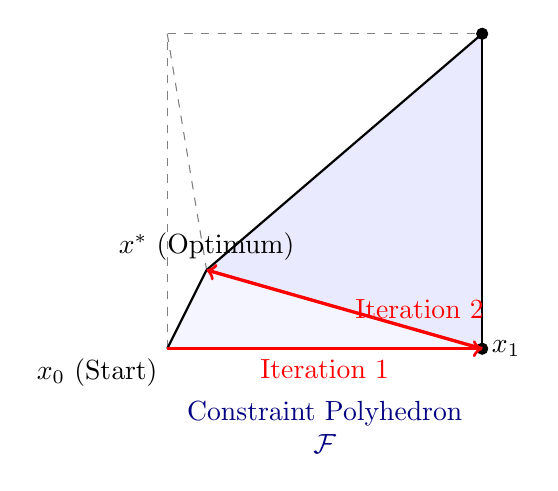
\begin{tikzpicture}[scale=2, z={( -0.3, -0.2)}, line join=round]
    \coordinate (A) at (0,0,0);
    \coordinate (B) at (2,0,0);
    \coordinate (C) at (2,2,0);
    \coordinate (D) at (0,2,0);
    \coordinate (Top) at (1,1,2.5);
    
    \fill[blue!5, opacity=0.8] (A) -- (B) -- (Top) -- cycle;
    \fill[blue!10, opacity=0.8] (B) -- (C) -- (Top) -- cycle;
    
    \draw[dashed, gray] (A) -- (D) -- (C);
    \draw[dashed, gray] (D) -- (Top);
    
    \draw[thick, black] (A) -- (B) -- (C);
    \draw[thick, black] (B) -- (Top);
    \draw[thick, black] (A) -- (Top);
    \draw[thick, black] (C) -- (Top);
    
    \filldraw[black] (B) circle (1pt);
    \filldraw[black] (C) circle (1pt);
    
    \draw[->, red, very thick] (A) -- (B) node[midway, below] {Iteration 1};
    \draw[->, red, very thick] (B) -- (Top) node[midway, right] {Iteration 2};
    
    \node[below left] at (A) {$x_0$ (Start)};
    \node[right] at (B) {$x_1$};
    \node[above] at (Top) {$x^*$ (Optimum)};
    
    \node[blue!50!black, align=center] at (1, -0.5, 0) {Constraint Polyhedron \\ $\mathcal{F}$};
\end{tikzpicture}
\caption{Geometric visualization of the Simplex Method. The algorithm moves from vertex to vertex along the edges of the polyhedron until it finds the optimum.}
\label{fig:simplex-path}
\end{figure}

\begin{figureexplanation}
\textbf{Walking on the edges:}
The set of feasible points forms a polyhedron. The optimum is always located at a vertex (or a face).
The algorithm starts from a vertex $x_0$, looks at the adjacent edges, and chooses the one that decreases the cost function the fastest (the most negative reduced cost). It "slides" along this edge to the next vertex ($x_1$), and repeats the operation.
\end{figureexplanation}

\section{Overview of the Simplex Method}

\begin{algorithm}[H]
    \caption{One step of the Simplex Method}
    \SetAlgoLined
    Given: $\mathcal{B}$, $\mathcal{N}$, $x_B=B^{-1}b\geq 0$, $x_N=0$\;
    Solve $B^\top\lambda = c_B$ for $\lambda$\;
    Compute $s_N=c_N - N^\top\lambda$\; \Comment{Pricing}
    \If{$s_N\geq 0$}{
        \Stop \Comment{optimal point found}
    }
    Select $q\in\mathcal{N}$ with $s_q<0$ as entering index\;
    Solve $Bd=A_q$ for $d$\;
    \If{$d\leq 0$}{
        \Stop \Comment{problem is unbounded}
    }
    Compute $x_q^+=\min_{i \mid d_i> 0}\left(\frac{(x_B)_i}{d_i}\right)$, use $p$ to denote the minimizing index $i$\;
    Update $x_B^+=x_B - d x_q^+$, $x_N^+=(0, \ldots, 0, x_q^+, 0, \ldots, 0)^\top$\;
    Change $\mathcal{B}$ by adding $q$ and removing the basic variable corresponding to column $p$ of $B$\;
\end{algorithm}

\section{Implementation and Practical Aspects}

The simplex algorithm presented above is conceptual. Its efficient and robust implementation requires addressing several critical points (see Nocedal \& Wright, Chapter 13).

\subsection{Linear Algebra and Revised Simplex}
In practice, explicitly computing the inverse of the basis $B^{-1}$ is computationally expensive and unstable. The \textbf{revised simplex} method instead maintains a factorization of the basis (often LU) which is updated at each iteration.
\begin{itemize}
    \item \textbf{Multipliers computation (Pricing):} We solve the linear system $B^\top \lambda = c_B$ to obtain $\lambda$, then we compute $s_N = c_N - N^\top \lambda$.
    \item \textbf{Displacement direction:} We solve the system $Bd = A_q$ to obtain the direction $d$.
\end{itemize}
These resolutions are fast if an up-to-date factorization of $B$ is available.

\subsection{Degeneracy and Cycling}
A basis is said to be \textbf{degenerate} if one or more basic variables are zero ($x_i = 0$ for $i \in \mathcal{B}$). 
In this case, the maximum possible step may be zero ($\alpha = 0$). The algorithm performs a basis change without changing the geometric point or improving the objective function.
If a sequence of such steps leads back to an already visited basis, the algorithm loops indefinitely: this is the phenomenon of \textbf{cycling}.
\begin{itemize}
    \item \textbf{Bland's Rule:} To avoid cycling, a simple rule is to always choose, among the candidates for entering (negative reduced cost) or leaving (minimum ratio), the one with the \textbf{smallest index}. This rule guarantees the termination of the algorithm.
\end{itemize}

\subsection{Initialization (Phase I and Phase II)}
The simplex algorithm requires an initial basic feasible solution. This is not always trivial to find. We often proceed in two phases:
\begin{itemize}
    \item \textbf{Phase I:} We introduce artificial variables $z$ and solve an auxiliary problem whose objective is to minimize the sum of these variables (for example, $\min \sum z_i$ subject to $Ax + Ez = b, x,z \ge 0$). If the minimum is 0, a feasible solution for the initial problem has been found.
    \item \textbf{Phase II:} We use the solution found in Phase I as a starting point to solve the original problem.
\end{itemize}

\bigskip
\begin{checkpoint}
\begin{itemize}
    \item \textbf{Geometry:} What does a basic feasible solution correspond to? (A vertex of the polyhedron).
    \item \textbf{Optimality:} Which vector must be positive to guarantee optimality? (Reduced costs).
    \item \textbf{Duality:} State the strong duality theorem.
\end{itemize}
\end{checkpoint}
